% Created 2024-08-03 Sat 16:24
% Intended LaTeX compiler: pdflatex
\documentclass[10pt]{article}
% =================================BASE====================================%
\usepackage[left=2cm,right=2cm,top=2cm,bottom=2cm]{geometry} % Marges
\usepackage[T1]{fontenc} % Nécessaire avec FrenchBabel
\usepackage[utf8]{inputenc} % Important pour symboles Francophones, é,à,etc
\usepackage{csquotes} % Recommandé par PDFLatex lors de la compilation. 

% Calligraphie
%\usepackage{pxfonts} % Met le texte ET les maths en Palatino + donne accès à des symboles math
%\usepackage{palatino} % Cette commande met seulement le texte en police palatino
\usepackage{lmodern} % Pour les maths? Lmodern pour les maths
\usepackage{cfr-lm}
% Use lmodern for sans-serif
\usepackage{mathrsfs} % Permet la command \mathscr (Lettres attachées genre) \mathscr(B)

% Bibliographie
%\usepackage[backend=bibtex,style=phys,sorting=ynt]{biblatex}
\usepackage[backend=biber,sorting=ynt,style=authoryear]{biblatex} % N'est pas utilisé par le compilateur org-mode, mais NÉCESSAIRE. Voir le fichier init.el pour changer le style. 
\addbibresource{master-bibliography.bib}


\usepackage{amsmath, amssymb, amsthm} % Symb. math. (Mathmode+Textmode) + Beaux théorèmes.
\usepackage{mathtools,cancel,xfrac} % Utilisation de boîtes \boxed{} + \cancelto{}{}, xfrac
\usepackage{graphicx, wrapfig} % Géstion des figures.
\usepackage{hyperref} % Permettre l'utilisation d'hyperliens.
\usepackage{color} % Permettre l'utilisation des couleurs.
\usepackage{colortbl} % Color tables
\usepackage[dvipsnames]{xcolor} % Couleurs avancées.

% Physique
\usepackage{physics} % Meilleur package pour physicien. 

% Style
\usepackage{lipsum} % For fun
\usepackage{tikz} % Realisation de figures TIKZ.
\usetikzlibrary{arrows.meta,bending} % Arrow heads 
\usepackage{empheq} % Boite autour de MULTIPLE équations
\usepackage{bbding}

% Français
\usepackage[french]{babel} % Environnements en Français.

\usepackage{titling} % Donne accès à \theauthor, \thetitle, \thedate

% ==============================BASE-(END)=================================%





% ================================SETTINGS=================================%
% Pas d'indentation en début de paragraphe :
\setlength\parindent{0pt}
\setlength{\parskip}{0.15cm}

% Tableaux/tabular
% Espace vertical dans les tabular/tableaux
\renewcommand{\arraystretch}{1.2}
% Couleur des tableaux/tabular
% \rowcolors{3}{violet!5}{}

% Couleurs de hyperliens :
\definecolor{mypink}{RGB}{147, 0, 255}
\hypersetup{colorlinks, 
             filecolor=mypink,
             urlcolor=mypink, 
             citecolor=mypink, 
             linkcolor=mypink, 
             anchorcolor=mypink}


% Numéros d'équations suivent les sections :
\numberwithin{equation}{section} 

% Les « captions » sont en italique et largeur limitée
\usepackage[textfont = it]{caption} 
\captionsetup[wrapfigure]{margin=0.5cm}

% Retirer l'écriture en gras dans la table des matières
\usepackage{tocloft}
\renewcommand{\cftsecfont}{\normalfont}
\renewcommand{\cftsecpagefont}{\normalfont}

% Change bullet style
\usepackage{pifont}
\usepackage{enumitem}
%\setlist[itemize,1]{label=\ding{224}}
\setlist[itemize,1]{label=\ding{239}}
\renewcommand{\boxtimes}{\blacksquare}
% ================================SETTINGS=================================%



% ==============================NEWCOMMANDS================================%
% CQFD symbol
\renewcommand{\qedsymbol}{$\hfill\blacksquare$}

% Vecteurs de base :
\newcommand{\nvf}{\vb{\hat{n}}}
\newcommand{\evf}{\vb{\hat{e}}}
\newcommand{\ivf}{\vb{\hat{i}}}
\newcommand{\jvf}{\vb{\hat{j}}}
\newcommand{\kvf}{\vb{\hat{k}}}
\newcommand{\uu}{\vb{u}}
\newcommand{\vv}{\vb{v}}
\newcommand{\ust}{\vb{u}_{\ast}}

% Physics empty spaces 
\newcommand{\short}{\vphantom{pA}}
\newcommand{\tall}{\vphantom{pA^{x^x}_p}}
\newcommand{\grande}{\vphantom{\frac{1}{xx}}}
\newcommand{\venti}{\vphantom{\sum_x^x}}
\newcommand{\pt}{\hspace{1pt}} % One horizontal pt space

% Moyenne numérique entre deux points de grilles. 
\newcommand{\xmean}[1]{\overline{#1}^x}
\newcommand{\ymean}[1]{\overline{#1}^y}
\newcommand{\zmean}[1]{\overline{#1}^z}
\newcommand{\xymean}[1]{\overline{#1}^{xy}}

% Tilde over psi
\newcommand{\tpsi}{\tilde{\psi}}
\newcommand{\tphi}{\tilde{\phi}}

% Nota Bene env : (\ding{89})
%\newcommand{\nb}{$\boxed{\text{\footnotesize\EightStarConvex}\pt \mathfrak{N. B.}}$\hspace{4pt}}
\newcommand{\nb}{\underline{{\footnotesize\EightStarConvex}\pt $\mathfrak{N.B.}$\vphantom{p}}\hspace{3pt}}

\newcommand{\exemple}{
\parbox[center]{2.2cm}{\begin{tcolorbox}[sharp corners, rounded corners=northeast, rounded corners=southeast,
colback=Violet!2, colframe=black,
size=small, width=2cm, left=-0.25pt, bottom=-0.5pt,
arc is angular, arc=2.5mm, boxrule=0.35pt, leftrule=4pt, %bottomrule=1pt,
after={\enskip}] Exemple \end{tcolorbox}}}

\newcommand{\rad}{\text{Rad}}


\newcommand{\cqfd}{\hfill$\blacktriangleleft$}

% Define the nota bene environment
\usepackage{tcolorbox}
\newtcolorbox{notabene}{
     colback=blue!5,
     colframe=black,
     boxrule=0.5pt,
     arc=2pt,
     left=5pt,
     right=5pt,
     top=5pt,
     bottom=5pt,
}


\newcommand{\cmark}{\ding{52}}
\newcommand{\xmark}{\ding{55}}
% ==============================NEWCOMMANDS================================%



% ==============================PAGE-TITRE=================================%
% Titlepage 
\newcommand{\mytitlepage}{
\begin{titlepage}
\begin{center}
{\Huge \thesubtitle \par}
\vspace{2cm}
{\Huge \MakeUppercase{\thetitle} \par}
\vspace{2cm}
RÉALISÉ DANS LE CADRE\\ D'UN PROJET POUR \par
\vspace{2cm}
{\Huge ISMER--UQAR \par}
\vspace{2cm}
{\thedate}
\end{center}
\vfill
Rédaction \\
{\theauthor}\\
\url{charles-edouard.lizotte@uqar.ca}\\
ISMER-UQAR\\
Police d'écriture : \textbf{CMU Serif Roman}
\end{titlepage}
}
% ==============================PAGE-TITRE=================================%



% =================================ENTÊTE==================================%
\usepackage{fancyhdr}
\pagestyle{fancy}
\setlength{\headheight}{13pt}
\renewcommand{\headrulewidth}{0.025pt} % Ligne horizontale en haut

\fancyhead[R]{\textit{\thetitle}}
\fancyhead[L]{\ \thepage}
\fancyfoot[R]{\textit{\theauthor}}
\fancyfoot[L]{}
\fancyfoot[C]{} 
% =================================ENTÊTE==================================%
\author{Charles-Édouard Lizotte}
\date{04/08/2023}
\title{Carnet de bord, Université McGill}
\newcommand{\thesubtitle}{Contrat Été 2023}
\hypersetup{
 pdfauthor={Charles-Édouard Lizotte},
 pdftitle={Carnet de bord, Université McGill},
 pdfkeywords={},
 pdfsubject={},
 pdfcreator={Emacs 29.4 (Org mode 9.7.8)}, 
 pdflang={French}}
\begin{document}

\mytitlepage
\tableofcontents\newpage
\section{Retour sur les murs, test et problèmes rencontrés -- \textit{<2023-07-31 Mon>}}
\label{sec:org3703370}

Après une semaine bien mouvementée, j'ai réussi à faire fonctionner le modèle \emph{shallow water} veituré par des murs.
En fin de semaine, j'ai profité de l'occasion pour réaliser une batterie de test.
Principalement, les lignes horizontales qui \emph{sabotaient} le modèle périodique --solvé par algorithme \emph{multigrid} -- sont encore et toujours là.
J'ai été extrêmement surpris et déçu par leur retour.
J'avais la certitude que le problème venait d'une boucle de rétroaction dans MUDPACK avec la constante d'intégration qui devenait de plus en plus grande, faisant réduire la valeur relative de la solution réelle par rapport à la solution fournie par MUDPACK.
En changeant les frontières pour des conditions Dirichlet, j'estimais donc que constante d'intégration disparaîtrait, réglant du même coup tous nos problèmes.\bigskip

Malheureusement, ce ne fut pas le cas.
Mentionnons que MUDPACK semble trouver des solutions raisonables (voir figure \ref{fig:org8f33188}), mais qu'on observe toujours les lignes horizontales à l'intérieur de la divergence de la première couche.

\begin{center}
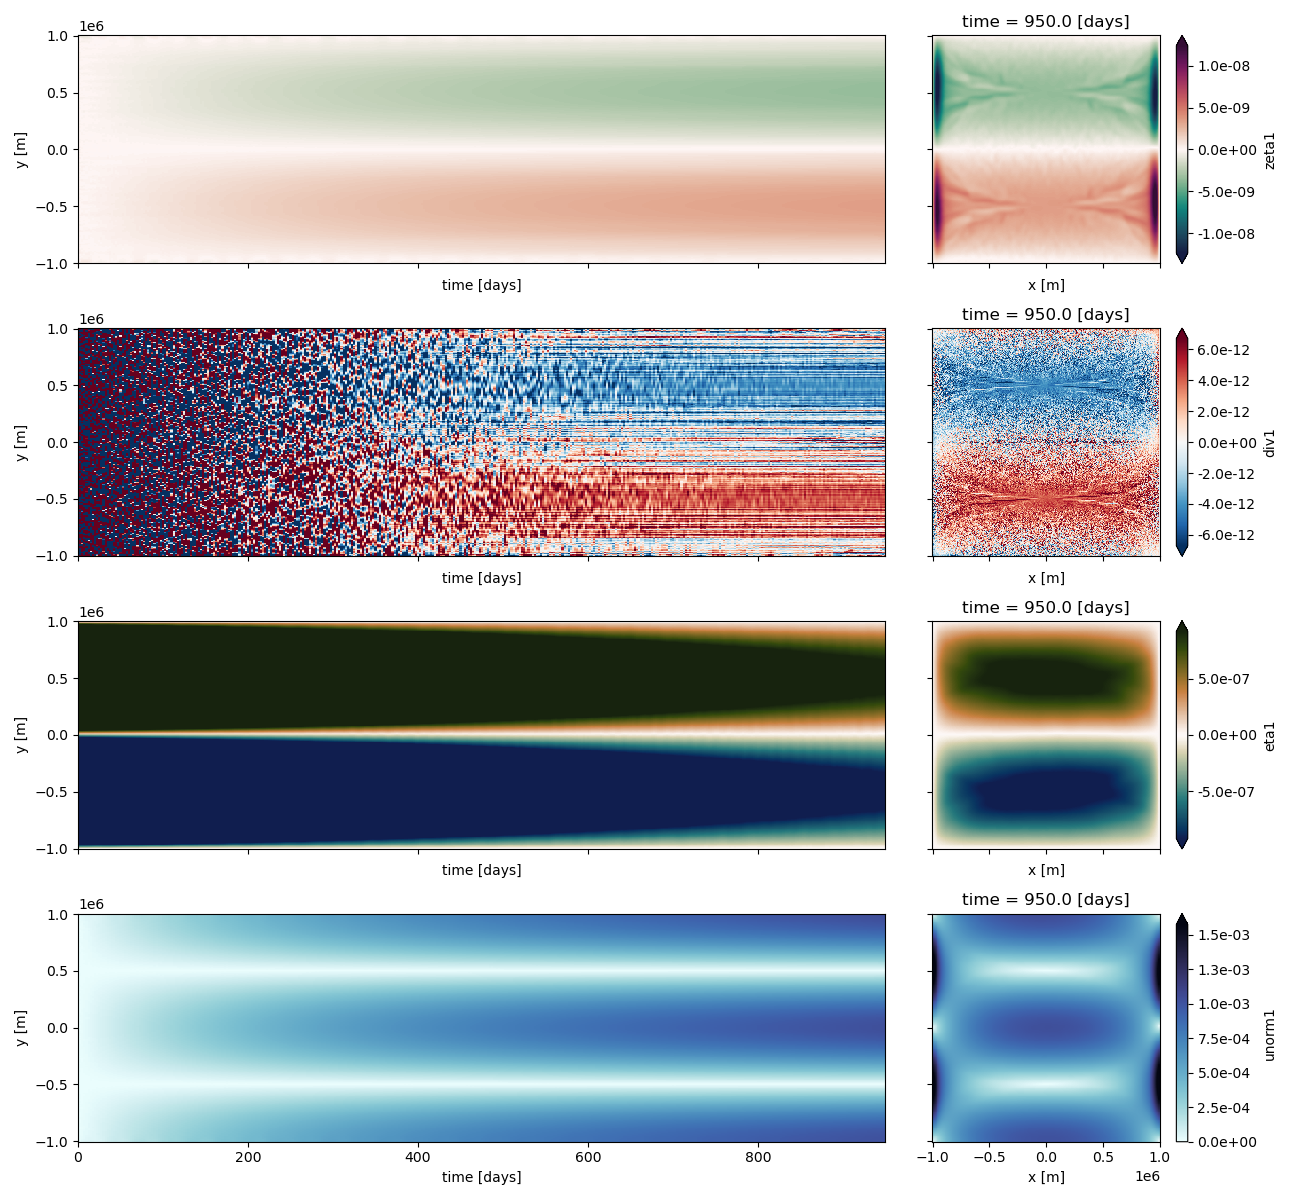
\includegraphics[width=.9\linewidth]{figures/tests/2023-07-31_hovmoller1_t=950days.png}
\caption{\label{fig:org8f33188}Test avec modèle borné par des murs.}
\end{center}
\newpage
\section{Quelques pistes de solution}
\label{sec:org0cc8ea9}
Avant tout, souvenons nous des discussions que nous avons eu avec David : 
Pour observer ce genre de comportement, il doit absolument exister une \textbf{partie divergente} à notre courant \textbf{qui survit entre chaque itération}.
À chaque pas de temps, on advecte notre partie non-divergente (avec MUDPACK) sans se soucier de la partie divergente cachée dans les courante \(u\) et \(v\).
Essentiellement, la partie divergente survit car on ne corrige pas le courant.
\subsection{Retirer la partie divergente après quelques timesteps -- \textit{<2023-08-01 Tue>}}
\label{sec:org24f76cb}
C'est la solution qui avait été proposée par David et Louis-Philippe.
Quand nous avions des conditions frontières périodiques, cette option était \textbf{catastrophiquement peu efficace}.
Comme mentionné plus haut, la solution calculée par MUDPACK avait toujours une constante d'intégration, ce qui signifiait que la solution calculée avait quelques ordres de grandeur de plus que la solution réelle.
Ce processus augmentait drastiquement l'erreur relative sur la solution réelle et les résultats étaient très douteux.\bigskip

Bien qu'un problème similaire pourrait se produire avec MUDPACK -- en ce qui attrait à l'erreur relative, cette option est toujours sur la table.\bigskip

\nb \emph{Si les autres méthodes proposée plus bas échouent, nous allons retenter le coup parce que je serai désespéré.}
\subsection{Rendre le bruit initial non-divergent \textit{<2023-07-31 Mon>}}
\label{sec:org24c5851}
\textbf{Cet idée m'a été révélée dans un rêve.}
Concrétement, le bruit initial (fortement divergent d'ailleurs) ne fait que croître au long de notre série temporelle (comme on peut l'observer dans le diagramme de Hovmoller pour la divergence, figure \ref{fig:org8f33188}).
La question qu'on doit ici se poser est maintenant formullée : « Est-ce qu'un bruit définit comme non-divergent à la base aurait le même effet? »\bigskip

Bref, ça vaut la peine de vérifier.
Si c'est le cas, ça signifie que notre modèle périodique fonctionnait et qu'on s'en faisait pour rien.
Il me semble raisonnable de croire que, au fond, le modèle ne pouvait tout simplement pas se débarrasser lui-même de la partie divergente.\bigskip

\textit{<2023-08-01 Tue> } J'ai testé tout ça.
Bien que je crois que la pratique derrière ce concept soit bonne, le résultat reste le même, les lignes horizontales dans les divergences persistent.
Donc, on va garder le module qui produit un bruit non-divergent, mais ça ne change pas grand chose, malheureusement.

\begin{figure}[htbp]
\centering
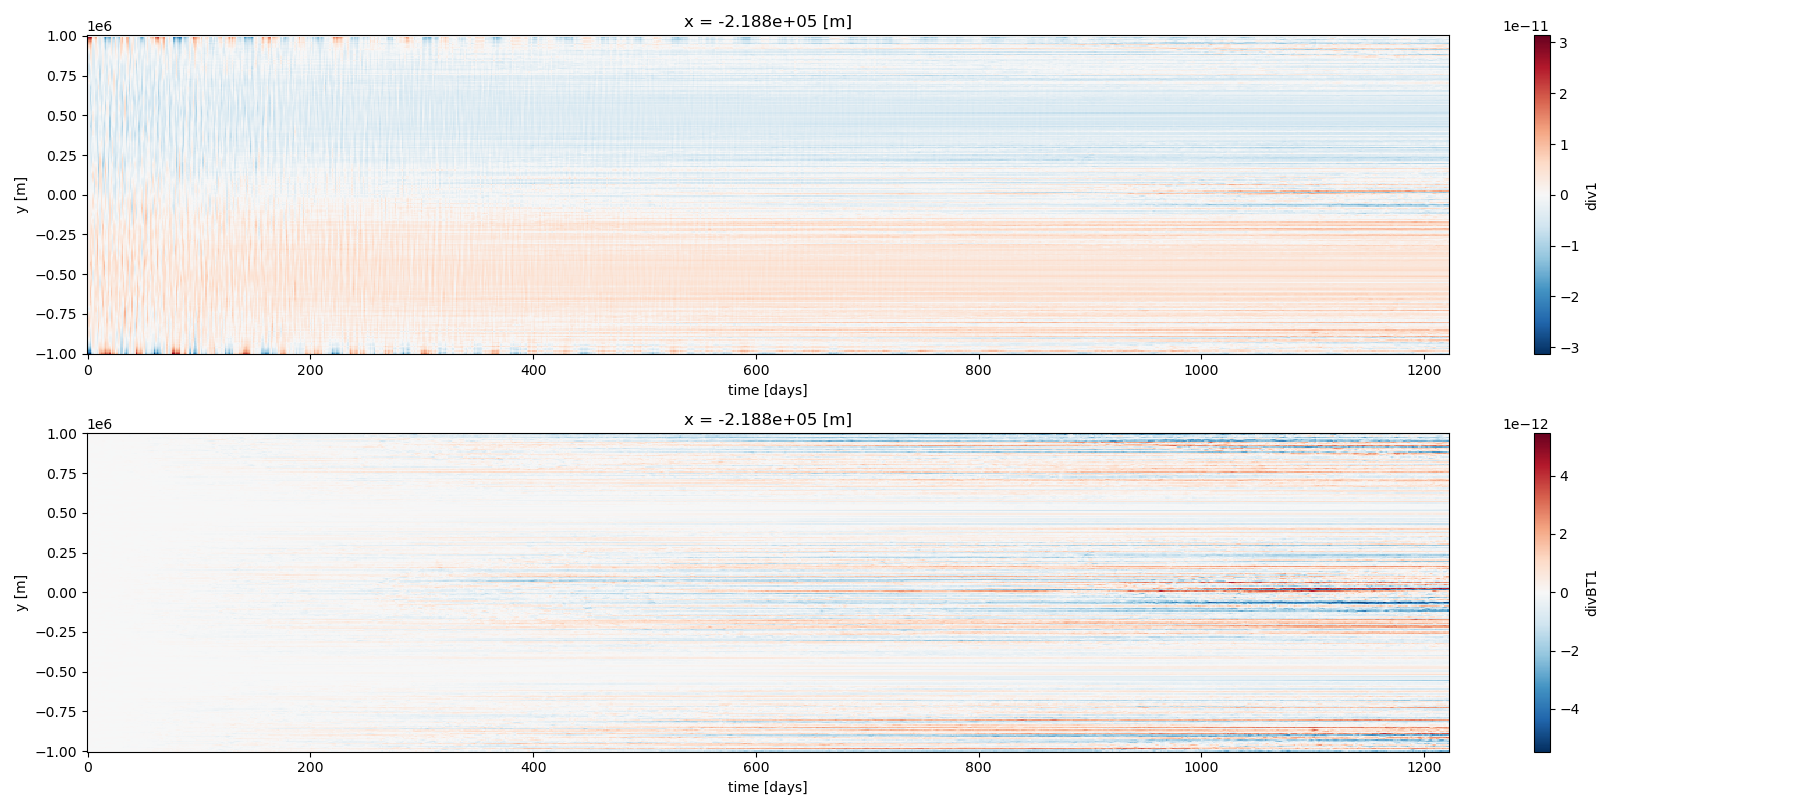
\includegraphics[width=.9\linewidth]{figures/debuggage/2023_08_03_comp_divergences.png}
\caption{Diagrammes de Hovmollet comparant la divergence barotrope et la divergence dans la première couche du modèle.}
\end{figure}

Les « lignes horizontales » apparaissent à la fois dans la divergence de toutes les couches, ainsi que dans la divergence barotrope.
Ceci nous laisse croire que le problème pourrait se retrouver ailleurs que dans MUDPACK.
Mentionnons aussi que je croyais que le problème disparaîtrait avec les conditions frontières Dirichlet.
Donc, je crois qu'il faut revenir à mon intuition initiale, soit que des erreurs \textbf{non-corrigées se transmettent dans la partie barocline} de notre RHS.\bigskip

\nb \emph{Pour faire preuve d'intelligence, il serait intéressant de vérifier une fois de plus que le RHS de u trouvé à l'aide de MUDPACK est non-divergent.
Ensuite, vérifier que le tout (u et v) sont eux-même non-divergents.}
\subsection{Améliorer la précision de MUDPACK comme proposée dans la documentation -- \textit{<2023-08-03 Thu>}}
\label{sec:org03d091d}

\subsubsection{Argument mathématique proposé dans la documentation}
\label{sec:org444a74d}
Concrètement, la méthode proposée dans la documentation se résume ainsi :
Assumons une équation différentielle partielle de la forme
\begin{equation}
   \mathscr{L}\qty{\pt p(t)\pt} = r(t),
\end{equation}
où \(\mathscr{L}\) est un opérateur linéaire quelconque et \(r(t)\) est le \emph{RHS} de ce dernier.\bigskip

Cette équation est valide à tous moments, ainsi
\begin{equation}
   \mathscr{L}\qty{\pt p(t+\delta t)\pt} = r(t+\delta t),
\end{equation}

En assumant que la solution à \(t+\delta t\) aura une forme similaire à celle à \(t\), on pourrait se permettre de définir un écart \(e(t,\delta t)\) entre les deux solutions, de sorte que
\begin{equation}
\label{eq:org8454ed3}
   e(t,\delta t) = p(t+\delta t) - p(t).
\end{equation}

Donc, il est simple de voir que l'opérateur linéarie satisfera
\begin{equation}
   \mathscr{L}\qty{\pt e(t,\delta t)} = r(t+\delta t) - r(t).
\end{equation}

Pour les conditions frontières Neumann, représentées par les fonction \(f(t)\) et \(f(t+\delta t)\), dont défnies comme
\begin{align}
   && \pdv{}{x} \qty[ \tall p(t) ] = f(t), && \pdv{}{x} \qty[\tall p(t+\delta t)] = f(t+\delta t). &&
\end{align}
Ainsi, les conditions frontière Neumann pour la correction sont données par
\begin{equation}
   \pdv{}{x} \qty[ \tall e(t,\delta t) ]  = f(t+\delta t) - f(t).
\end{equation}

Pour des contions frontières Dirichlet, on soustrait \(p(t)\) à \(p(t+\delta t)\), de sorte à suivre l'équation \ref{eq:org8454ed3}, soit
\begin{equation}
   \eval{e(t,\delta t)\ }_{x_0} = \eval{ \qty{ \pt p(t+\delta t) - p(t)\pt \tall } }_{x_0}.
\end{equation}

Dans notre cas, la condition Dirichlet est que \(p(t)\) est nul aux murs pour tous \(t\), ainsi \(e(t,\delta t)\) aussi sera nulle partout.\bigskip

\nb \emph{Mentionnons aussi que nous n'appliquons cette méthode pour le RHS barotrope et non le courant barotrope. Nous y reviendrons peut-être dans la section suivante.}
\subsubsection{Tests de la méthode, résultats et conclusion -- \textit{<2023-08-02 Wed>}}
\label{sec:org158c775}
J'ai testé la méthode et elle m'amène exactement les mêmes résultats qu'avant.
Bien que ça peut paraître \emph{anti-climatique}, je suis heureux parce que ça me renseigne sur deux choses :
\begin{itemize}
\item \textbf{Le problème ne vient définitivement pas de MUDPACK}.
Si c'était le cas, tous les changements qu'on a réalisés pour optimiser la résolution, soient :
\begin{enumerate}
\item Passer de solver \(\psi_{BT}\) à \(\delta \psi_{BT}\);
\item Ensuite, solver \(\Delta (\delta \psi_{BT})\) au lieu \(\delta\psi\).
\item Retirer la partie divergente à chaque 1000 pas de temps.
\end{enumerate}

\item Et puis, ça veut dire que je n'ai \textbf{pas fait d'erreurs en modifiant l'algorithme} -- ce qui m'aurait pris pas mal de temps à débugger.
\end{itemize}
\section{Retour à la correction totale, mais avec la méthode proposée dans la documentation}
\label{sec:org47dd584}

Essentiellement, on utilise la méthode proposée dans la section précédente, mais sur tous \(\psi\).
En gros,
\begin{enumerate}
\item On décompose notre courant mis à jour, soit \(\tilde{\uu}\), en parties barotropes (\(\tilde{\uu}_{BT}\) et baroclines (\(\tilde{\uu}_{BC}\)) ;
\item On trouve le rotationnel de la partie barotrope du courant;
\begin{equation}
   \tilde{\zeta}_{BT} = \kvf\cdot\curl(\tilde{\uu}_{BT});
\end{equation}
\item On soustrait la nouvelle partie barotrope à l'ancienne, de sorte à avoir un \(\delta \zeta_{BT}\).
\begin{equation}
   \delta \zeta_{BT} = \tilde{\zeta}_{BT} - \zeta_{BT}^t;
\end{equation}
\item À l'aide de MUDPACK, on trouve la différence entre la nouvelle et l'ancienne fonction de courant barotrope \(\delta \psi_{BT}\);
\begin{equation}
   \delta \psi_{BT} = MUDPACK \pt \qty(\delta \zeta_{BT},\pt \laplacian{});
\end{equation}
\item On additionne avec l'ancienne partie barotrope pour avoir la nouvelle, soit
\begin{equation}
   \psi^{t+1}_{BT} = \tilde{\psi}_{BT} = \psi^{t} + \delta \psi_{BT}.
\end{equation}
\item On trouve le courant barotrope \(\uu^{t+1}_{BT}\) à l'aide de
\begin{equation}
   \uu^{t+1}_{BT} = \kvf\times\gradient(\psi^{t+1}_{BT})
\end{equation}
\end{enumerate}
\subsection{Débuggage de la méthode proposée dans la documentation -- \textit{<2023-08-08 Tue>}}
\label{sec:orgd4c2021}

Commmençons par tester le modèle \emph{shallow water} à 2 couche, ensuite nous pourrons voir si les erreurs se transmettent aux couches inférieures.
D'un côté, le temps de calcul sera grandement réduit et nous verrons s'il y a une corrélation avec l'épaisseur des couches, étant donné que nous n'avons qu'une seule couche.\bigskip

On se rappelle que les équations \emph{shallow water} à solver sont exprimées par
\begin{equation}
   \pdv{\uu_k}{t} = \qty(\zeta_k + f\pt) \pt \kvf\times\uu_k -\frac{\gradient|\uu_k^2|}{2}  -\frac{\gradient{P_k}}{\rho_k} - \frac{\gradient p_{surf}}{\rho_k},
\end{equation}
où \(P_k\) est la pression à la couche \(k\) et \(g'_k\) est la  \textbf{gravité réduite} , respectivement illustrés par 
\begin{align}
   && P_k = \qty(\sum_i^{k-1} P_i ) + \rho_1 g'_k \eta_k &&  \text{et} && g'_k = g \pt\qty(\frac{\rho_k - \rho_{k-1}}{\rho_1})\ . &&
\end{align}

\nb \emph{Juste en regardant ça, j'ai remarqué que le modèle de Tianze n'avait tout simplement pas définit le ratio des rho. Ce qui n'est pas très grave comme les rho entre les couches sont proches. Je les ai rajoutés pour m'assurer que tout soit bon.}\bigskip
\subsection{Problème précédent avec la divergence? -- \textit{<2023-08-11 Fri>}}
\label{sec:org9855a9d}
Déjà, le problème de divergence barotrope est \textbf{disparu complétement}.
Donc l'objectif de la section précédente est une réussite.
Par contre, on voit des trucs \emph{funky}, comme on peut le constater dans les prochaines sections.
\subsection{Premier test -- \textit{<2023-08-09 Wed>}}
\label{sec:orgb5082ff}

Les paramètres sont illustrés dans le tableau suivant :

\begin{center}
\begin{tabular}{llrl}
\hline
\hline
Paramètres & Symbole & Valeur & Unité\\
\hline
Taille du domaine & L\textsubscript{x} = L\textsubscript{y} & 2000 & km\\
Nombre de points de grilles & nx = ny & 513 & --\\
Pas de temps & \(\Delta\) t & 300 & s\\
Paramètre de Coriolis & f & 7\texttimes{}10\textsuperscript{-5} & s\textsuperscript{-1}\\
Paramètre beta & beta & 1\texttimes{}10\textsuperscript{-11} & m\textsuperscript{-1}s\textsuperscript{-1}\\
Amplitude du vent & \(\tau\)\textsubscript{atm} & 0.1 & N m\textsuperscript{-2}\\
Coefficient de visc. biharmonique & A\textsubscript{bh} & dx\textsuperscript{4} \texttimes{}10\textsuperscript{-5} & s\textsuperscript{-1}\\
Coefficient de frottement & r\textsubscript{drag} & 10\textsuperscript{-7} & s\textsuperscript{-1}\\
Vitesse des ondes internes barocliniques & c\textsubscript{bc} & 2 & ms\textsuperscript{-1}\\
Épaisseur de la couche supérieure & H\textsubscript{1} & 1000 & m\\
Épaisseur de la couche inférieur & H\textsubscript{2} & 1000 & m\\
\hline
\end{tabular}
\end{center}
\subsubsection{Détection d'une erreur majeure -- \textit{<2023-08-11 Fri>}}
\label{sec:org408948d}
Alors, il semble que j'avais mal calculé le laplacien au mur et ça pourrait être la source de nos troubles.
Juste pour s'en rappeler, il est possible de développer les deux points les plus proches du mur à l'aide de séries de Taylor.
\begin{align}
   (A)\hspace{1cm}&u(1) = u(0) + \qty(\frac{\Delta x}{1!}) \eval{\qty(\pdv{u}{x})\pt}_{\pt x=0} \ \pt+ \qty(\frac{\Delta x^2}{2!}) \eval{\qty(\pdv[2]{u}{x})\pt }_{\pt x=0} \\
   (B)\hspace{1cm}&u(2) = u(0) + \qty(\frac{2\Delta x}{1!}) \eval{\qty(\pdv{u}{x})\pt}_{\pt x=0} + \qty(\frac{4\Delta x^2}{2!}) \eval{\qty(\pdv[2]{u}{x})\pt }_{\pt x=0}.
\end{align}

On peut par la suite faire \((B) - 2(A)\), pour obtenir
\begin{equation}
   \eval{\qty(\pdv[2]{u}{x})\pt }_{\pt x=0} = \frac{(u(2) - 2u(1) )}{\Delta x^2 }
\end{equation}

Et l'on applique cette méthode partout, voir fonction \emph{laplacian\textsubscript{bndy.f90}}, en cas de doute.
\subsubsection{Résultats}
\label{sec:orge167305}
On voit une circulation semblable à celle des deux gyres de Stommel se développer autours de 50 à 100 jours.
Par la suite, une circulation constituée entièrement de tourbillons géostrophiques se développe sur l'ensemble du domaine.

\begin{center}
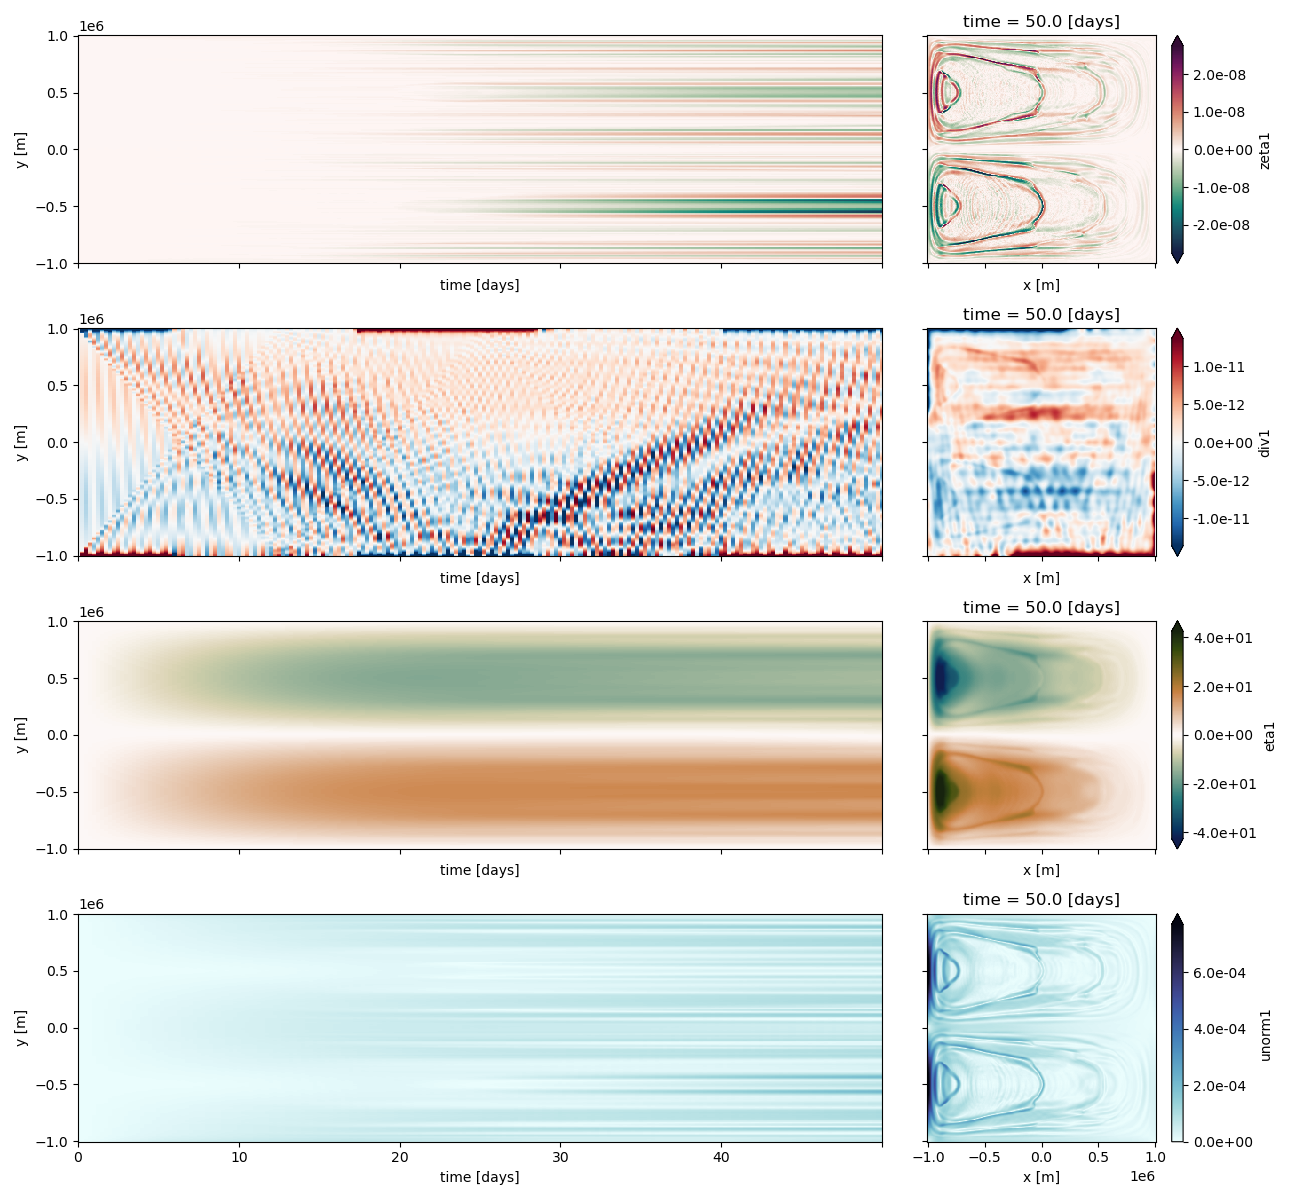
\includegraphics[width=.9\linewidth]{figures/tests/2023-08-14_hovmoller1_t=50days.png}
\end{center}
\begin{center}
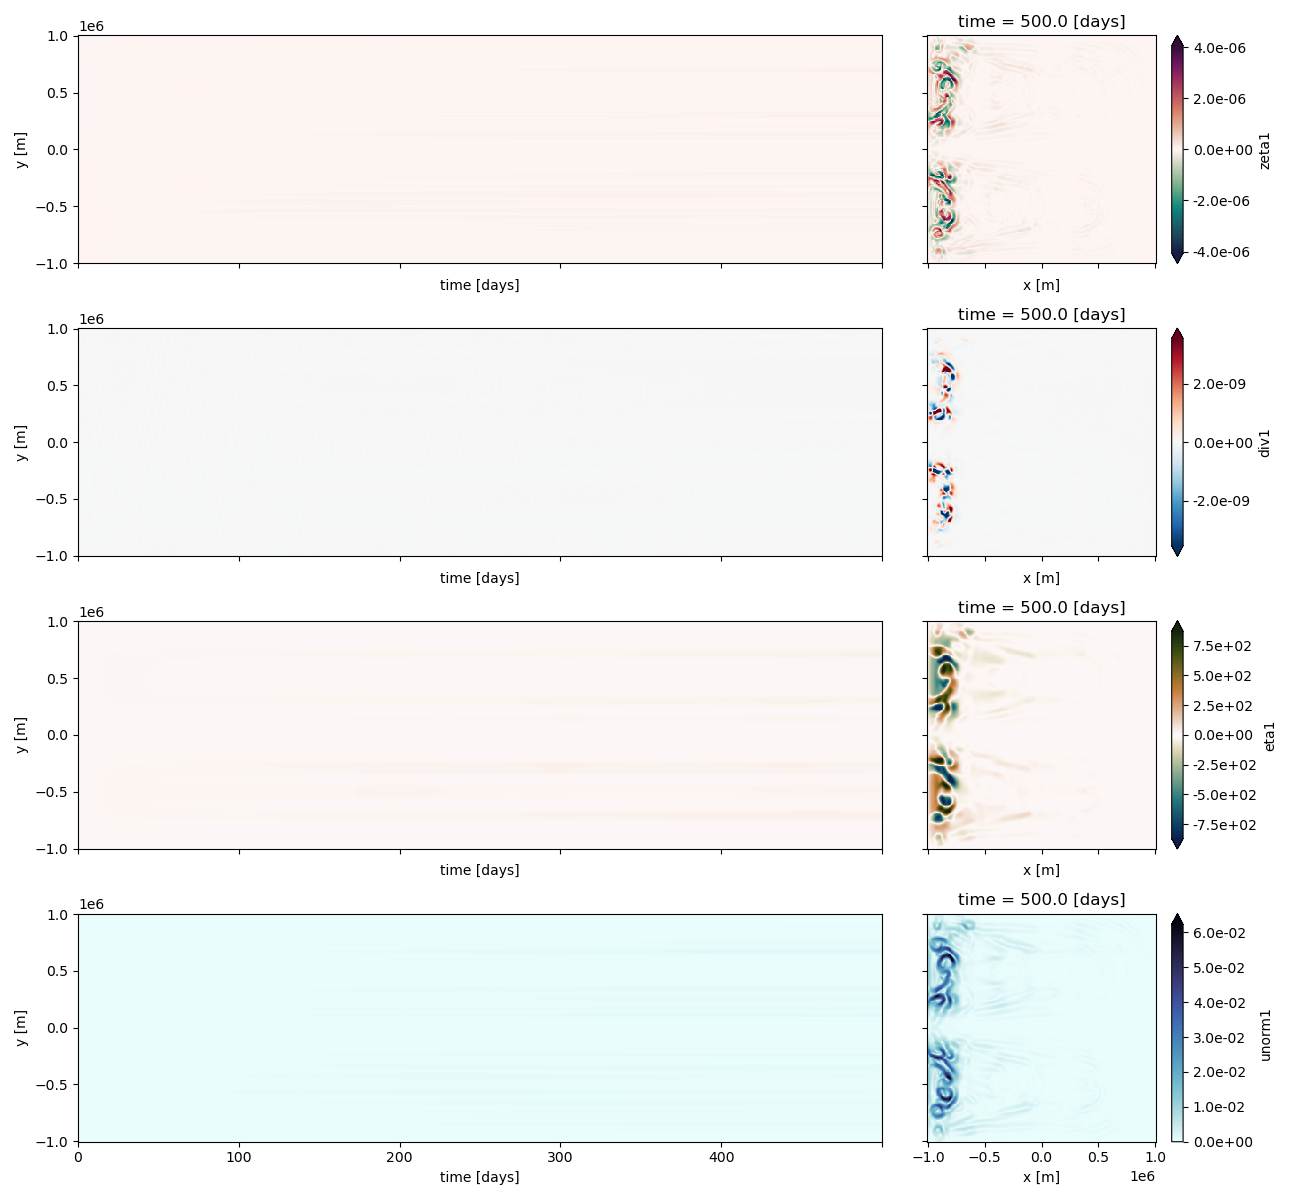
\includegraphics[width=.9\linewidth]{figures/tests/2023-08-14_hovmoller1_t=500days.png}
\end{center}
\begin{center}
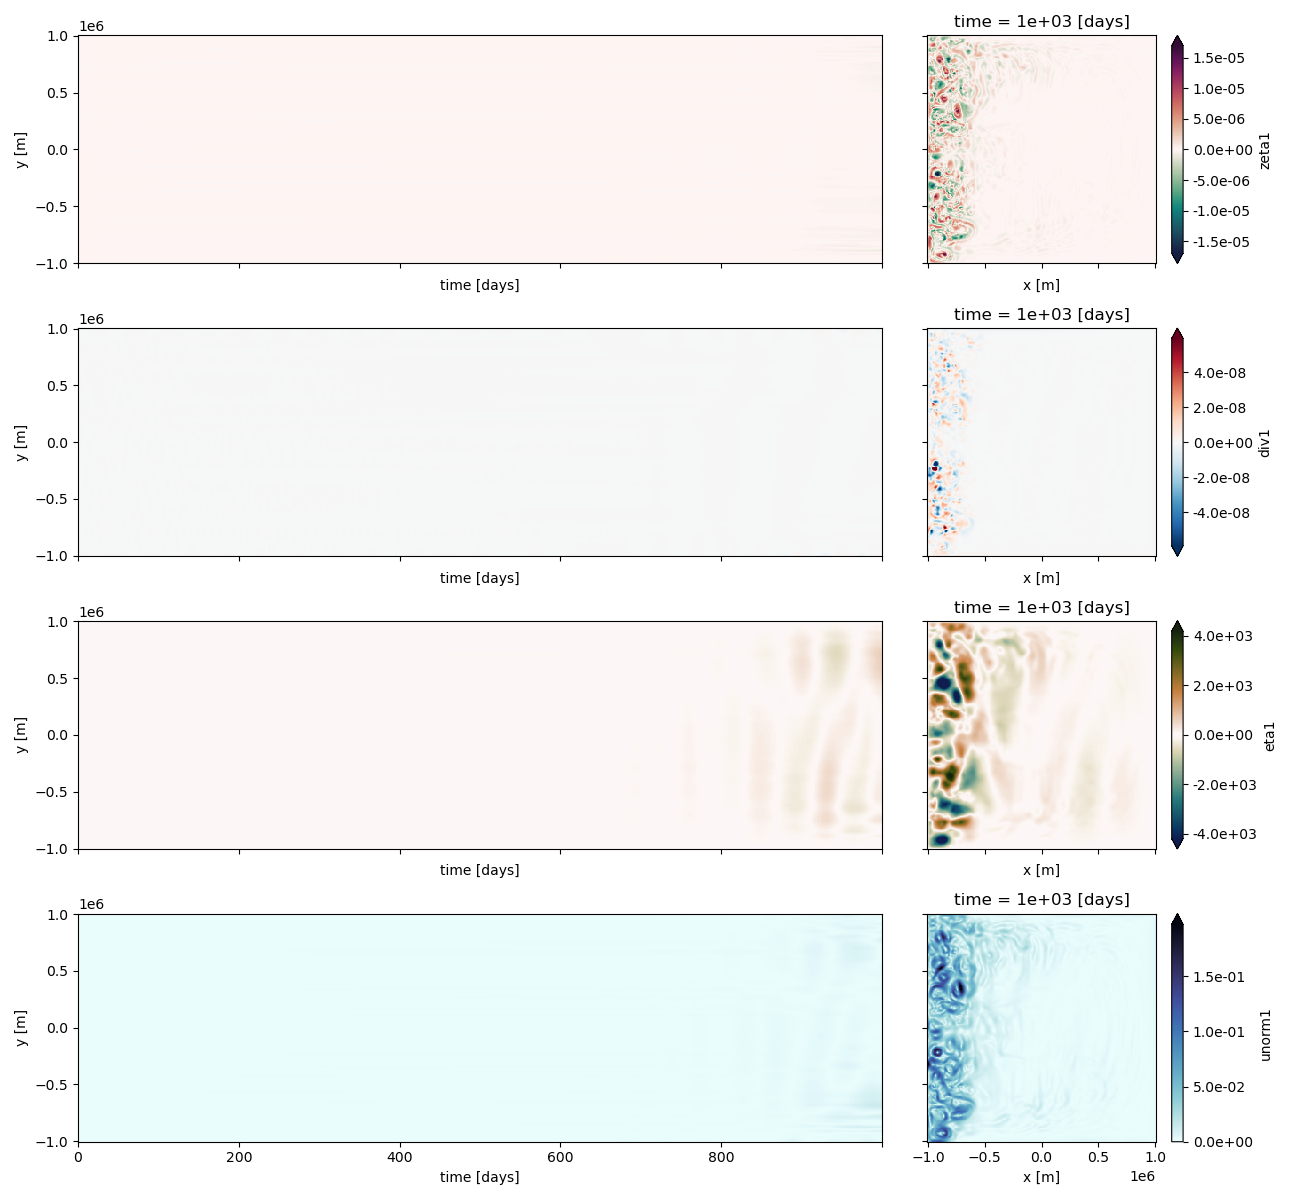
\includegraphics[width=.9\linewidth]{figures/tests/2023-08-14_hovmoller1_t=1000days.png}
\end{center}
\begin{center}
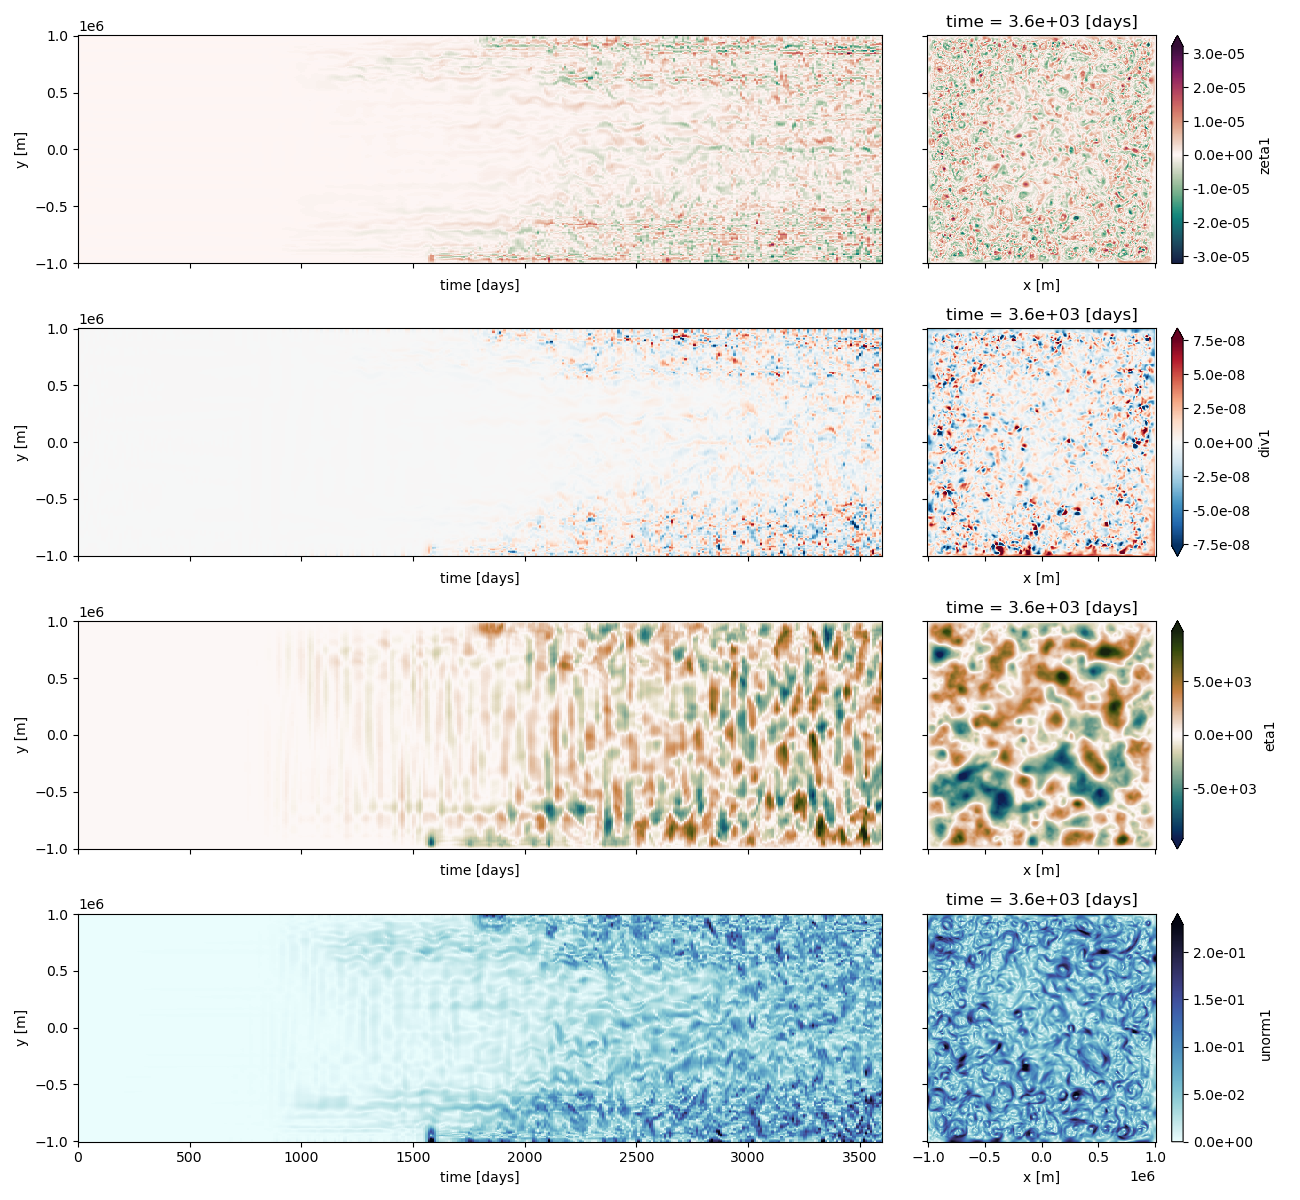
\includegraphics[width=.9\linewidth]{figures/tests/2023-08-14_hovmoller1_t=3600days.png}
\end{center}
\end{document}
